
\section{Alimentação} % (fold)
\label{sec:alimentação}
	
	O sistema de alimentação pode ser dividido em 2 grandes grupos: \textit{Bateria} e \textit{Carregador}, os quais estão descritos nas sub-seções dispostas a seguir.

	\subsection{Bateria de íon-lítio (Li-Ion)} % (fold)
	\label{sub:bateria}
		
		De todos os tipos de baterias esta é, sem dúvida, a melhor. Suas vantagens são diversas e variadas e não é justamente por isso que elas são empregadas em larga escala nos novos eletrônicos.

		Não-tóxicas, com capacidade de carga duas vezes maior que as de Ni-MH e três vezes maior que as de NiCd, sem efeito memória (ou seja, a bateria não vai “viciar”) e também mais leves, afinal o lítio é um dos metais mais leves já conhecidos. A densidade do lítio também permite a criação de baterias com maior capacidade.

		Outro ponto que dá muito mais vantagens às baterias de Li-Ion é o fato de estas baterias dispensarem ciclos completos de cargas, ou seja, não é necessário esperar a carga acabar para carregá-la novamente e quando carrega não precisa esperar que ela seja preenchida por completo. Além disso, ao estar carregada por completo a bateria cessa automaticamente o recebimento de energia para evitar sobrecargas.

		Estas baterias, porém, demandam um cuidado maior por parte de seus usuários, como por exemplo, a não exposição a altas temperaturas que podem causar danos definitivos e até mesmo sua explosão.

	\subsubsection{Bateria utilizada}

		A 18650 é uma bateria de 4.2V e possui 8.8Ah. É de Li-íon assim como as baterias de celular, no entanto possuindo maior capacidade energética. A figura \ref{img:bateria} mostra a bateria NK 18650.

		\begin{figure}[H]
			\centering
			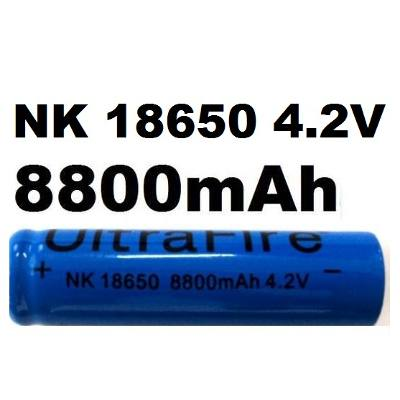
\includegraphics[scale=0.7]{figuras/bateria.jpg}
			\caption{Bateria NK 18650 Ultrafire.}
			\label{img:bateria}
		\end{figure}

		O Li-ion tem melhor relação de peso e potência que as baterias de Ni-MH ou Ni-Cd, tendo apenas o problema da tensão ser mais elevada.

		Usando o princípio da associação de fontes de tensão, resultará em um somatório das tensões das fontes. Quando 3 baterias de 4.2V são associadas em série temos o equivalente a um bateria de 12.6V, internamente em uma bateria é possível distinguir 3 células de 4.2V. Mas é preciso atentar que para resultar neste somatório todas as células ou fontes tem de estar com as polaridades sempre entre positivo para negativo ou vice versa.

	\subsubsection{Consumo energético}

		Foi realizada uma relação de consumo e capacidade de energia dos componentes para a escolha da bateria ideal, onde os motores consomem a maior parte da corrente.

		\begin{table}[H]
		\centering
		\caption{Consumo energético.}
		\label{tab:consumo_energético}
		\begin{tabular}{lllll}
		Componente               & Quantidade & Corrente unitária (mA) & Corrente total (mA) & Tensão (V) \\ \hline
		Ponte H                & 1          & 36                     & 36                  & 6          \\ \hline
		AtMega                 & 1          & 500                    & 500                 & 5          \\ \hline
		Motor DC               & 3          & 470                    & 1410                & 6          \\ \hline
		Módulo ESP8266         & 1          & 1000                   & 1000                & 3.3        \\ \hline
		Motor DC \\ 12V Aspiração & 1           & 4400                   & 4400                & 12         \\ \hline
		TOTAL                  &            &                        & 7421                & \\ \hline          
		\end{tabular}
		\end{table}

		De acordo com a tabela \ref{tab:consumo_energético}, é possível analisar a corrente e tensão de cada componente utilizado no projeto. Os componentes utilizados trabalharão com uma média de 7Ah, sendo que, um dos requisitos do robô é ter de aspirar um cômodo de maneira autônoma durante 30 minutos, com isto a corrente diminui para 3.5Ah.


	% subsection bateria (end)

	\subsection{Carregador} % (fold)
	\label{sub:carregador}
	
		Uma das grandes dificuldades na aplicação do sistema de alimentação em um projeto de eletrônico portátil é a forma com que se vai fornecer os ciclos de carga ao aparelho. No que tange as especificidades do nosso projeto, por ser um aspirador de pó que opera de forma autônoma, o maior desafio foi encontrar uma maneira de fazer com que o robô, após notar a necessidade, se dirigisse a sua base e começasse a se recarregar da forma mais simples e prática possível. 

Depois de diversas pesquisas e muitas hipóteses consideradas, chegou-se em consenso de que o princípio de carregamento por indução eletromagnética é o que mais se adequa ao nosso caso, já que não é necessário a conexão de cabos/conectores.

A indução eletromagnética consiste basicamente no surgimento de uma corrente elétrica oriunda de um fluxo magnético próximo de um condutor. O conceito é antigo e teve o princípio do raciocínio em 1820, quando Hans Christian Oesterd descobriu que cargas elétricas em movimento davam origem a um campo magnético.

 Tal descoberta levou diversos estudiosos da época a creer que o inverso também deveria ser possível de acontecer, ou seja: a varição do campo magnético levaria a uma produção de corrente elétrica. Michael Faraday, também dinamarquês, em 1931, batizou esse comportamento como indução eletromagnética e comprovou tal teoria através daquela que é conhecida até hoje com a Lei de Faraday.

 \begin{figure}[H]
	\centering
	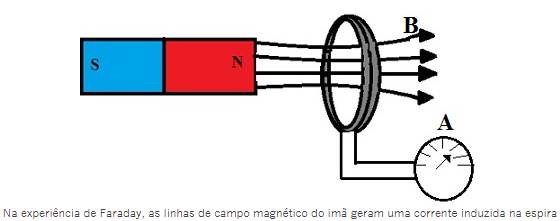
\includegraphics[scale=0.7]{figuras/carregador_inducao}
	\caption{Experiência de Faraday.}
	\label{img:faraday}
\end{figure}

A Lei de Faraday diz que uma força eletromotriz é produzida por condutores elétricos que se movimentam num campo magnético uniforme, ou então por um campo magnético variável. Tem uma melhor exemplificação da seguinte forma:


	$Fem = \frac{-d \phi }{dt}$


Sendo Fem a força eletromotriz (V), $\phi$ o fluxo magnético e t o tempo. Algum tempo depois James Clerk Maxwell, analisando o experimento de Faraday, escreveu uma outra lei que relaciona os campos elétrico e magnético, como podemos ver abaixo:


	$\nabla xE = \frac{-dB}{dt}$


Sendo $\nabla$ o operador nabla, E o campo elétrico e B o campo magnético. Analisando essa formulação conclui-se que o rotacional do campo elétrico é igual ao oposto da variação do campo magnético no tempo.


Esse conceito já é frequentemente utilizado em transformadores elétricos, motores, máquinas de indução em geral que hoje também englobam os carregadores mais modernos, afim de fornecer correntes de carga para baterias, especialmente para aparelhos como notebooks, tablets, smartphones e  e etc.

 \begin{figure}[H]
	\centering
	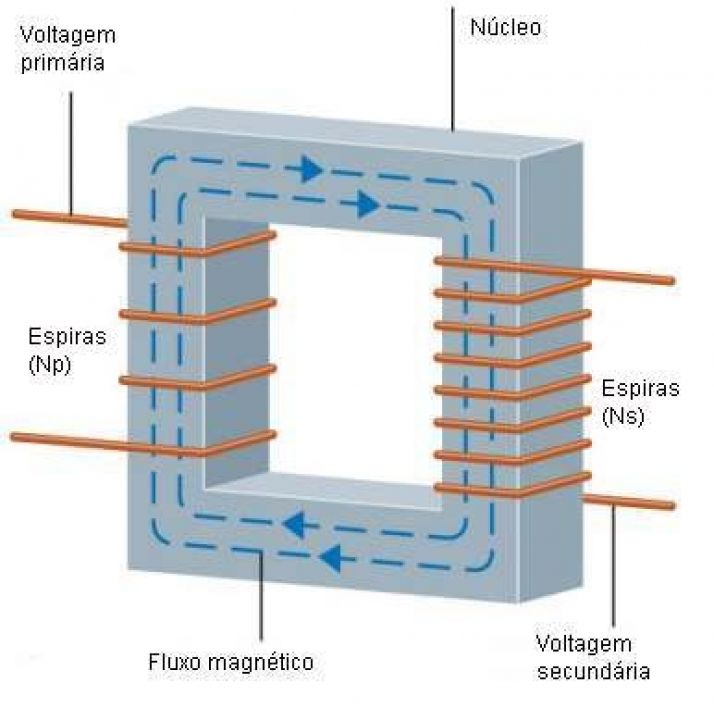
\includegraphics[scale=0.5]{figuras/transformador}
	\caption{Transformador elétrico.}
	\label{img:transformador}
\end{figure}

 \begin{figure}[H]
	\centering
	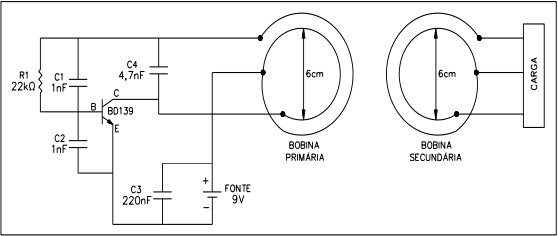
\includegraphics[scale=0.5]{figuras/diagrama_eletrico}
	\caption{Diagrama elétrico.}
	\label{img:diagrama_eletrico}
\end{figure}

Tendo como base experimentos já realizados que visaram a construção de um carregador por indução eletromagnética de forma artezanal, o grupo decidiu que deveríamos agir com a mesma linha de pensamento afim de ter o carregador para o projeto.

A construção demandou o uso de 3 capacitores, 1 resistor, 1 transistor, vários indutores (bobinas) e uma fonte de tensão contínua afim de se obter um circuito semelhante ao demonstrado na última figura.


	% subsection carregador (end)
% section alimentação (end)